        \subsubsection{Échelle linéaire à linéaire}
			\begin{question}{8,1219}{Transformation d'échelle}{2}{}
				Quelle est la formule générale permettant de passer de l'échelle du haut (abscisse $x$) à l'échelle du bas (abscisse $y$)? Par exemple, l'étoile rouge a pour coordonnées: $x=\num{-9.5}$ ou $y=\num{-11.5}$. Puisque les échelles sont linéaires, on cherche une relation du type $y = ax+b$ avec $a,b\in\R$.
				\begin{figure}
					\centering
					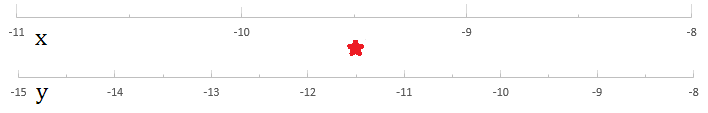
\includegraphics[scale=.75]{Antoine/Figures_Antoine/lin_-11_-8_to_lin_-15_-8_star_-9d5_-11d5.png}
				\end{figure}
			\end{question}
			\begin{reponses}
				\item[true] $y = 7(x+8)/3-8$
				\item[false] $y = 7(x-8)/3+8$
				\item[false] $y = 7x/3-8$
				\item[false] $y = 8/3-8x+7$
			\end{reponses}
			%%%%%%%%%%%%%%%%%%%%
			\begin{question}{8,1219}{Transformation d'échelle}{2}{}
				Quelle est la formule générale permettant de passer de l'échelle du haut (abscisse $x$) à l'échelle du bas (abscisse $y$)? Par exemple, l'étoile rouge a pour coordonnées: $x=\num{-9.5}$ ou $y=\num{7.5}$. Puisque les échelles sont linéaires, on cherche une relation du type $y = ax+b$ avec $a,b\in\R$.
				\begin{figure}
					\centering
					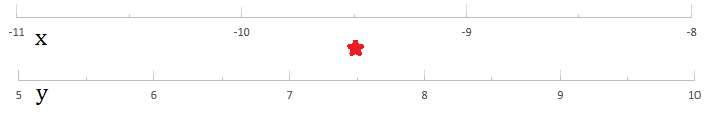
\includegraphics[scale=.75]{Antoine/Figures_Antoine/lin_-11_-8_to_lin_5_10_star_-9d5_7d5.png}
				\end{figure}
			\end{question}
			\begin{reponses}
				\item[true] $y = 5/3\times x+70/3$
				\item[true] $y = 5(x+14)/3$
				\item[false] $y = 3(x+70)/5$
				\item[false] $y = 3x/5+70$
			\end{reponses}
			%%%%%%%%%%%%%%%%%%%%
			\begin{question}{8,1219}{Transformation d'échelle}{2}{}
				Quelle est la formule générale permettant de passer de l'échelle du haut (abscisse $x$) à l'échelle du bas (abscisse $y$)? Par exemple, l'étoile rouge a pour coordonnées: $x=3$ ou $y=\num{14}$.
				\begin{figure}
					\centering
					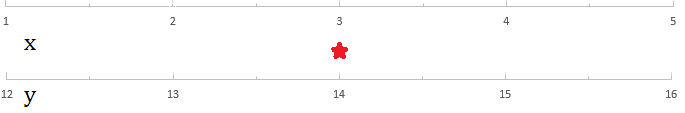
\includegraphics[scale=.75]{Antoine/Figures_Antoine/lin_1_5_to_lin_12_16_star_3_14.png}
				\end{figure}
			\end{question}
			\begin{reponses}
				\item[true] $y = x + 11$
				\item[false] $y = 14/3\times x+12$
				\item[false] $y = 12x-1$
				\item[false] $y = x + 12$
			\end{reponses}
			%%%%%%%%%%%%%%%%%%%%
			\begin{question}{8,1219}{Transformation d'échelle}{2}{}
				Quelle est la formule générale permettant de passer de l'échelle du haut (abscisse $x$) à l'échelle du bas (abscisse $y$)? Par exemple, l'étoile rouge a pour coordonnées: $x=5$ ou $y=\num{7.5}$. Puisque les échelles sont linéaires, on cherche une relation du type $y = ax+b$ avec $a,b\in\R$.
				\begin{figure}
					\centering
					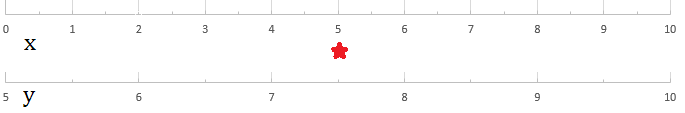
\includegraphics[scale=.75]{Antoine/Figures_Antoine/lin_0_10_to_lin_5_10_star_5_7d5.png}
				\end{figure}
			\end{question}
			\begin{reponses}
				\item[false] $y = 3x$
					\item[false] $y = 1/3\times x+5$
					\item[false] $y = 2 x-5$
					\item[true] $y = \num{0.5}x + 5$
			\end{reponses}
			%%%%%%%%%%%%%%%%%%%%
			\begin{question}{8,1219}{Transformation d'échelle}{3}{}
				Quelle est la formule générale permettant de passer de l'échelle du haut (abscisse $x$) à l'échelle du bas (abscisse $y$)? Par exemple, l'étoile rouge a pour coordonnées: $x=5$ ou $y=\num{14}$.
				\begin{figure}
					\centering
    	            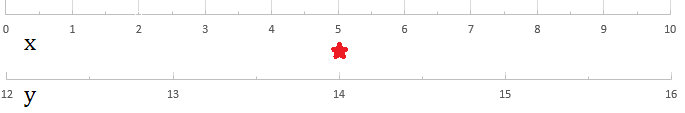
\includegraphics[scale=.75]{Antoine/Figures_Antoine/lin_0_10_to_lin_12_16_star_5_14.png}
				\end{figure}
			\end{question}
			\begin{reponses}
				\item[false] $y = 7x+0$
				\item[true] $y = 2/5\times x+12$
				\item[false] $y = \num{2.5}\times x-12$
				\item[false] $y = \num{5}x + 14$
			\end{reponses}
			%%%%%%%%%%%%%%%%%%%%
        \subsubsection{Échelle linéaire à logarithmique}
			\begin{question}{8,1219,1211,1222,1227}{Transformation d'échelle}{2}{}
				Quelle est la formule générale permettant de passer de l'échelle du haut (abscisse $x$) à l'échelle du bas (abscisse $y$)? Par exemple, l'étoile rouge a pour coordonnées: $x=\num{3}$ ou $y\simeq\num{2}$. Puisque l'on passe d'une échelle linéaire à une échelle logarithmique, on cherche une relation du type $y = a10^{bx}$ avec $a,b\in\R$.
				\begin{figure}
					\centering
					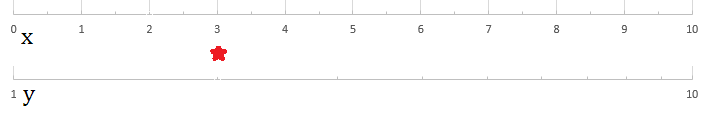
\includegraphics[scale=.75]{Antoine/Figures_Antoine/lin_1_10_to_log_1_10_star_3_2.png}
				\end{figure}
			\end{question}
			\begin{reponses}
				\item[false] $y = 10^{10x+1}$
				\item[false] $y = 10^{10x}$
				\item[true] $y = 10^{\num{.1}x}$
				\item[false] $y = 10\times 10^{10x}$
			\end{reponses}
			%%%%%%%%%%%%%%%%%%%%
			\begin{question}{8,1219,1211,1222,1227}{Transformation d'échelle}{2}{}
				Quelle est la formule générale permettant de passer de l'échelle du haut (abscisse $x$) à l'échelle du bas (abscisse $y$)? Par exemple, l'étoile rouge a pour coordonnées: $x=\num{1000}$ ou $y=\num{-12}$. Puisque l'on passe d'une échelle logarithmique à une échelle linéaire, on cherche une relation du type $y = a\log_{10}(bx)$ avec $a,b\in\R$.
				\begin{figure}
					\centering
					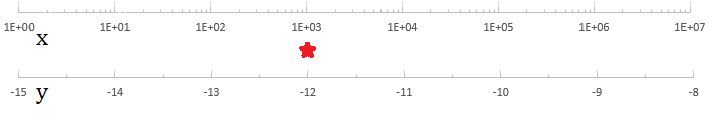
\includegraphics[scale=.75]{Antoine/Figures_Antoine/log_1_1e7_to_lin_-15_-8_star_1e3_-12.png}
				\end{figure}
			\end{question}
			\begin{reponses}
				\item[false] $y = 5\log_{10}(2x)$
				\item[false] $y = -15\log_{10}(10x)$
				\item[true] $y = -15+\log_{10}(x)$
				\item[false] $20\log_{10}(x)$
			\end{reponses}
			%%%%%%%%%%%%%%%%%%%%
        \subsubsection{Échelle logarithmique à logarithmique}
			\begin{question}{8,1219,1211,1222,1227}{Transformation d'échelle}{3}{}
				Quelle est la formule générale permettant de passer de l'échelle du haut (abscisse $x$) à l'échelle du bas (abscisse $y$)? Par exemple, l'étoile rouge a pour coordonnées: $x=\num{1e3}$ ou $y\simeq\num{2683}$. Puisque l'on passe d'une échelle logarithmique à une échelle logarithmique, on cherche une relation du type $y = a\log_{10}(bx)$ avec $a,b\in\R$.
				\begin{figure}
					\centering
					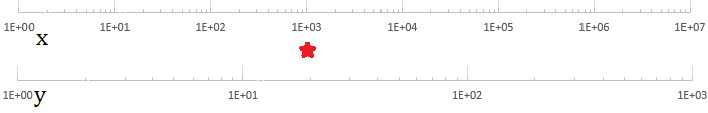
\includegraphics[scale=.75]{Antoine/Figures_Antoine/log_1_1e7_to_log_1_1e3_star_1e3_2e1.png}
				\end{figure}
			\end{question}
			\begin{reponses}
				\item[true] $y = x^{8/7}$
				\item[false] $y = 7/8\log_{10}(x)$
				\item[false] $y = x^{\num{7/8}}$
				\item[false] $\log_{10}(y) = \num{7}\log_{10}(x) + 8$
			\end{reponses}
			%%%%%%%%%%%%%%%%%%%%
			\begin{question}{8,1219,1211,1222,1227}{Transformation d'échelle}{3}{}
				Quelle est la formule générale permettant de passer de l'échelle du haut (abscisse $x$) à l'échelle du bas (abscisse $y$)? Par exemple, l'étoile rouge a pour coordonnées: $x=\num{4}$ ou $y=\num{2}$. Puisque l'on passe d'une échelle logarithmique à une échelle logarithmique, on cherche une relation du type $\log_{10}(y) = a\log_{10}(bx)$ avec $a,b\in\R$. Attention à bien faire le calcul, la réponse n'est peut-être pas si évidente (pensez à utiliser les propriétés des logarithmes et puissances).
				\begin{figure}
					\centering
					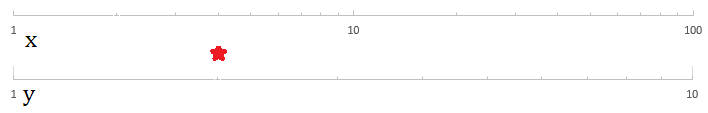
\includegraphics[scale=.75]{Antoine/Figures_Antoine/log_1_100_to_log_1_10_star_4_2.png}
				\end{figure}
			\end{question}
			\begin{reponses}
				\item[false] $y = \num{0.5}\log_{10}(x)$
					\item[false] $y = x^2+\num{0.5}$
					\item[false] $y = \num{10}\log_{10}(x) + 5$
					\item[true] $y = x^{\num{0.5}}$
			\end{reponses}
			%%%%%%%%%%%%%%%%%%%%
    %ajouter idées de MJ ramage (voir correction) + Loreynne
    %ajouter avec réaction https://www.techniques-ingenieur.fr/actualite/articles/8-reactions-chimiques-incroyables-2866/ mesurer la taille de la colonne après la réaction.
